% !Mode:: "TeX:UTF-8"
\chapter{如何使用本模板}
\label{chap:howtouse}

\section{关于本模板}
本模板\footnote{\href{https://github.com/PlainSailing/SDUThesis}{本模板Git仓库}}是在天津大学的~\LaTeX{}~毕业论文模板\footnote{\href{https://github.com/xnth97/TJUThesisLatexTemplate}{原始模板Git仓库}}的基础上修改完成的,其格式基本符合山东大学控制科学与工程学院学士学位论文的格式要求,但本人并不能保证完全符合,只是希望能通过自己的一点努力帮助大家都学会这款出色的排版系统的基本使用。到目前为止该模板应该是已开源的唯一一个针对山大控院本科生定制的~\LaTeX{}~模板,该模板与其他多数模板相比优点在于完全废弃了CJK宏包,在最新的TexLive2015(Windows7)套装下使用自带的编辑器TeXworks能顺利编译通过。编译时需要执行四次编译,通过xelatex+bibtex+xelatex+xelatex就可以生成带有完整目录和参考文献信息的PDF文档。编译时也可以使用命令行切换到当前目录下,然后执行Python脚本compile.py或者Windows批处理文件compile.bat来一次性完成,该脚本可以实现自动对过程文件的清理以及自动重复编译。关于LaTex的基本入门可以参考这篇文章\textcolor[rgb]{1.00,0.00,0.00}{\href{http://liam0205.me/2014/09/08/latex-introduction/}{始终-一份其实很短的 LaTeX 入门文档}}。
\section{基本输入示例}
文章的结构分为三个层次,分别是chapter、section、subsection,当你想要开始一个新的章节时,首先要新建一个文件保存在body文件夹下,并在sdumain.tex文件中通过$\backslash$include\{body/文件名\}的方式插入在合适的位置。一个新的章节应该以$\backslash$chapter\{章节名\}开头,同样section、subsection也是如此。之后就可以进行正常的文本输入工作了,要注意换行($\backslash\backslash$或$\backslash$newline)和重起一段(两个空行)的区别,在文本中输入的一个空行会被当做换行而不是换段处理。如果你需要修改封面内容,需要到preface文件夹下cover.tex文件里进行修改,如果需要修改论文题目可能就麻烦些,需要在setup文件夹下format.tex文件中大约第232行修改,并通过一些排版以适合自己的标题长度。
\section{数学输入示例}
行内公式使用$\backslash$(\textcolor[rgb]{0,0,1}{公式代码}$\backslash$)或者\$\textcolor[rgb]{0,0,1}{公式代码}\$来输入。这是一个行内公式$\mathop {\lim }\limits_{x \to \infty } \frac{x}{{\sin x}}$,行内公式能够紧凑的插入到文字中间,对行间距不产生影响。


行间公式使用$\backslash$[\textcolor[rgb]{0,0,1}{公式代码}$\backslash$]或者\$\$\textcolor[rgb]{0,0,1}{公式代码}\$\$来输入。这是一个行间公式$$\mathop {\lim }\limits_{x \to \infty } \frac{x}{{\sin x}}$$行间公式单独占一行。


使用数学环境$\backslash$begin\{equation\} \textcolor[rgb]{0,0,1}{公式代码} $\backslash$end\{equation\}可以输入带有编号的行间公式
\begin{equation} \label{eq:math1}
\mathop {\arg \max }\limits_{{\theta _0},{\theta _1},{\theta _2},\sigma } \ln L = \sum\limits_{i = 1}^n {\ln (\frac{1}{{\sqrt {2\pi {\sigma ^2}} }}{e^{\frac{{d{g_i} - ({\theta _0} + {\theta _1}v({x_i}) + {\theta _2}s({x_i}))}}{{2{\sigma ^2}}}}})} 
\end{equation}
数学环境还可以实现对公式的引用,公式(\ref{eq:math1})就是一个例子。


要注意的是,所有在数学环境包括行内行间公式里的字符都将被视为变量名来根据数学逻辑进行排版,空格空行将被忽略。如果需要输入普通文本应该使用$\backslash$textrm\{..\}来输入,比如$dg\textrm{ and dg}$,空格则用$\backslash$quad、$\backslash$qquad、$\backslash$,来输入。数学公式里的黑体用$\backslash$mathbf\{..\}输入,空心粗体用$\backslash$mathbb\{..\}输入,比如$\mathbf{R}\textrm{ and }\mathbb{R}$。至于数学公式可以用MathType工具排好之后直接复制过来,但是要先修改预置菜单里的剪切与复制预置选项以支持~\LaTeX{}~的语法。


\section{图片与表格插入}
\subsection{插入表格}
如\ref{tab:table1}所示,要插入这样一个表格。首先要开始一个表格环境$\backslash$begin\{table\}[htbp],参数含义为h(这里),t(顶部),b(底部),p(浮动体),设置标题$\backslash$caption\{BMI指数分类详表\}和字体。开始一个表格$\backslash$begin{tabular}\{c|cccc\},参数c表示居中显示对应列,参数|表示对应列之间用竖线分隔,真正的表格部分以$\backslash$toprule开始,输入列名后以$\backslash$midrule分割,接下来是数据部分,各列之间用\$分隔,各行之间用$\backslash\backslash$分隔,如果行与行直间需要用横线分隔使用$\backslash$hline命令,最后一个表格以$\backslash$bottomrule结束。
\begin{table}[htbp]
\caption{\textcolor[rgb]{1.00,0.00,0.00}{\href{http://baike.baidu.com/link?url=YDwxEa1gfVTHNICd8OjZG-YLsBgE4iFsy0UkQ-d4jVyln9tqov_jmFNlVwRD_sAB}{BMI指数分类详表}}}\label{tab:table1}
\vspace{0.5em}\centering\wuhao
\begin{tabular}{c|cccc}
\toprule[1.5pt]
BMI分类 & WHO标准 & 亚洲标准 & 中国参考标准 & 相关疾病发病的危险性\\
\midrule[1pt]
体重过低&<18.5&<18.5&<18.5&低(但其它疾病危险性增加)\\
\cline{3-4}
正常范围&18.5~24.9&18.5~22.9&18.5~23.9&平均水平\\
超重&≥25&≥23&≥24&增加\\
肥胖前期&25.0~29.9&23~24.9&24~26.9&增加\\
I度肥胖&30.0~34.9&25~29.9&27~29.9&中度增加\\
II度肥胖&35.0~39.9&≥30&≥30&严重增加\\
Ⅲ度肥胖&≥40.0&≥40.0&≥40.0&非常严重增加\\
\bottomrule[1.5pt]
\end{tabular}
\vspace{\baselineskip}
\end{table}
\FloatBarrier
\subsection{插入图片}
插入图片的方式和插入表格差不多,这里以在同一行插入一对图如图\ref{fig:subfig1}来示范一下。代码如下:
\begin{verbatim}
\begin{figure}[htbp]
  \centering
  \subfigure[处理前]{
            \label{fig:subfig1:subsubfig1}
            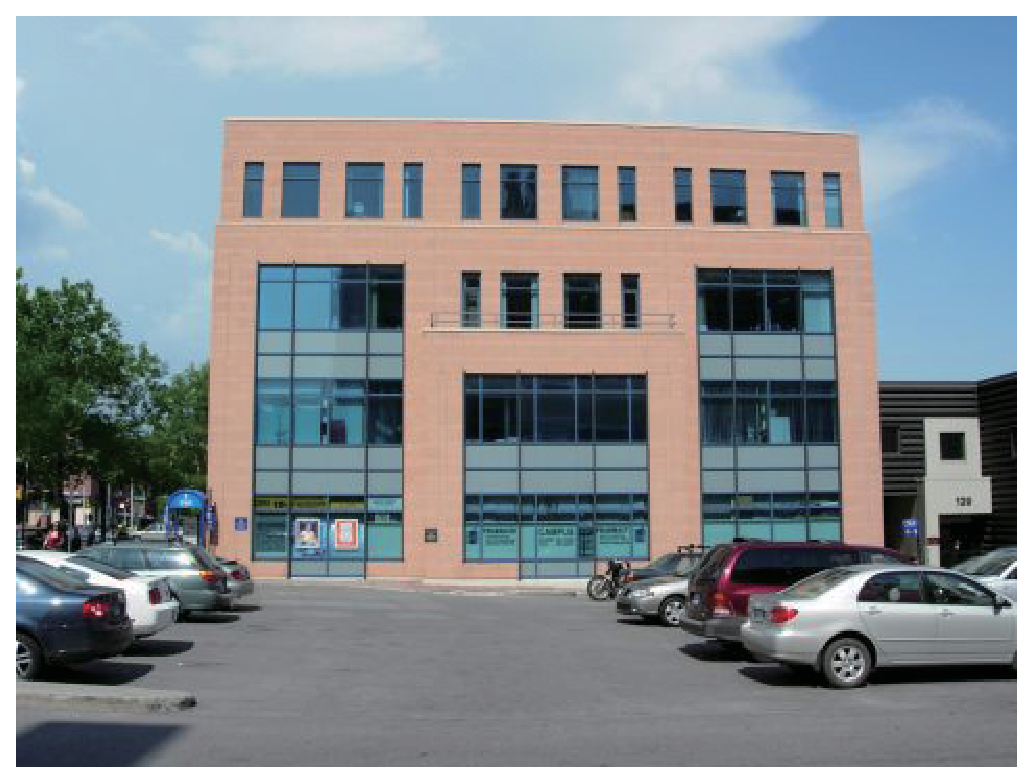
\includegraphics[width=0.4\textwidth]{figures/beforedeal}}
  \subfigure[处理后]{
            \label{fig:subfig1:subsubfig2}
            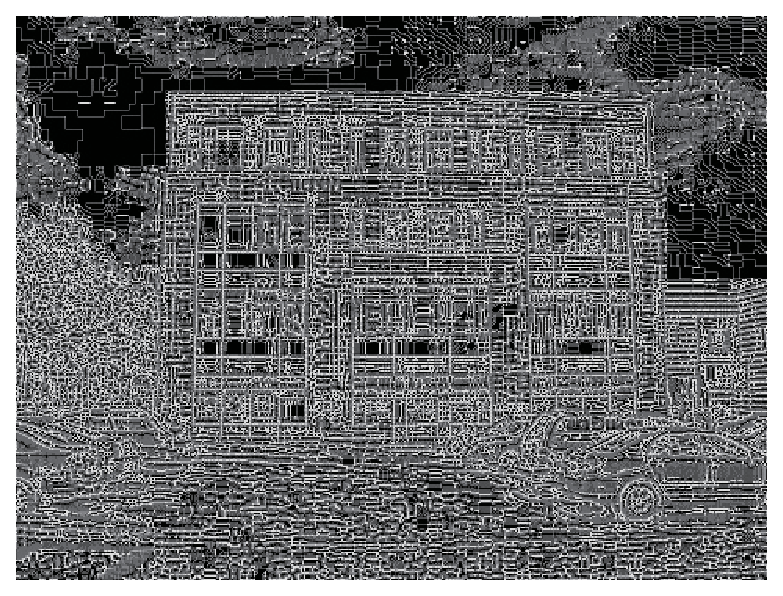
\includegraphics[width=0.4\textwidth]{figures/afterdeal}}
  \caption{处理效果}\label{fig:subfig1}
\vspace{\baselineskip}
\end{figure}
\end{verbatim}
\begin{figure}[htbp]
  \centering
  \subfigure[处理前]{
            \label{fig:subfig1:subsubfig1}
            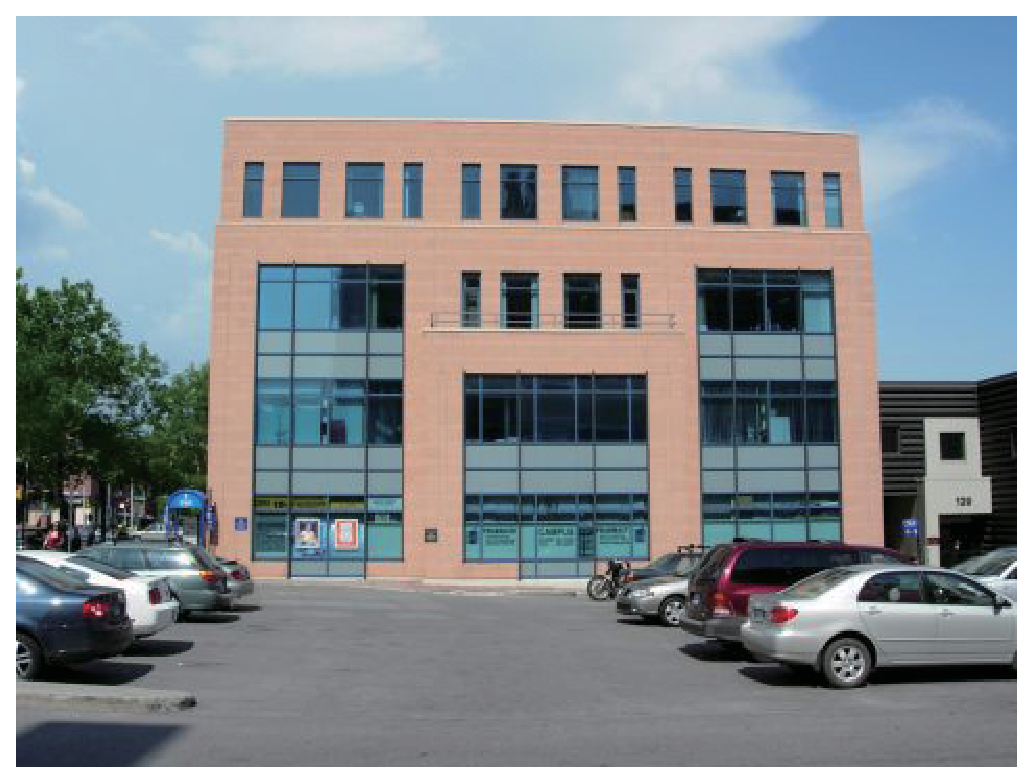
\includegraphics[width=0.4\textwidth]{figures/beforedeal}}
  \subfigure[处理后]{
            \label{fig:subfig1:subsubfig2}
            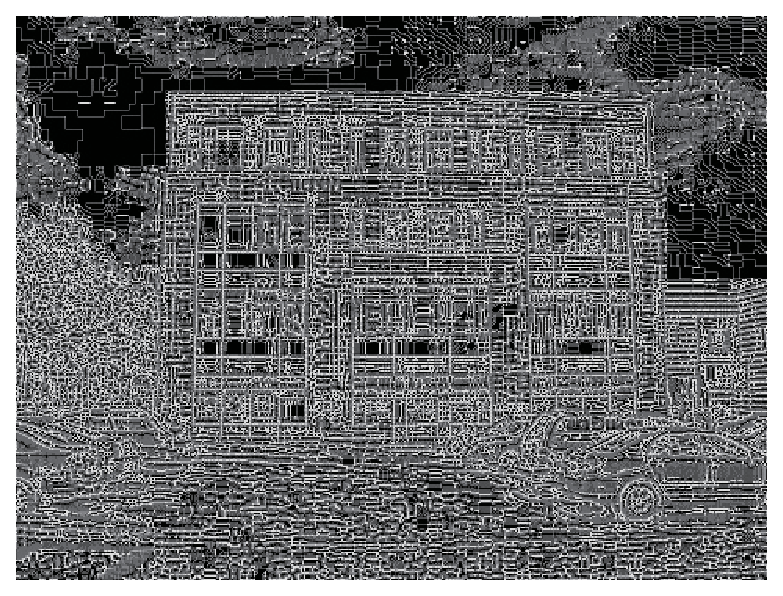
\includegraphics[width=0.4\textwidth]{figures/afterdeal}}
  \caption{处理效果}\label{fig:subfig1}
\vspace{\baselineskip}
\end{figure}